\documentclass[a4paper,12pt]{article}
\usepackage[english]{babel}
\usepackage[utf8]{inputenc}

\usepackage[top=2.5cm, bottom=2.5cm, left=2cm, right=2cm]{geometry}

\usepackage{datetime}
\newdateformat{monthyeardate}{%
  \monthname[\THEMONTH], \THEYEAR}

\usepackage{subcaption}

% Math packages
\usepackage{mathtools}
\usepackage{amsmath}
\usepackage{amsfonts}
\usepackage{amssymb}

\usepackage{enumitem}
\usepackage{algorithm}
\usepackage{algpseudocode}

\usepackage{listings}

\usepackage{makecell}

\usepackage[hidelinks]{hyperref}

\title{Mobile and Social Sensing Systems}
\author{Francesco Barbarulo, Giovan Battista Rolandi}
\date{\monthyeardate\today}

\begin{document}
\pagenumbering{roman}

\maketitle
\abstract{The aim of these notes is to give some pills of every argument for the oral test. We have assumed that the reader has attended the lessons because these notes, by themselves, are not sufficient to have a global and profound knowledge.

We wish you good luck!}

\tableofcontents

\newpage

\pagenumbering{arabic}

\section{Introduction}
\subsection{Mobility}
\begin{itemize}
    \item \textbf{Physical}: hardware actually changes its physical position;
    \item \textbf{Logical}: applications and data may need to be moved for design reasons.
\end{itemize}

Mobile computing relys on the ability to use devices \textit{non-physically connected} and \textit{context-aware}. And these devices must keep computinal and communicaiton capabilities paying attention to energy comsumption because of their battery-powered nature.

\section{Localization systems}
Localization systems consist of two main blocks:
\begin{enumerate}[label=(\roman*)]
	\item Set of deployed nodes with different \textit{states}:
		\begin{itemize}
		 	\item \textbf{beacon} (\textit{landmarks} or \textit{anchors}): already know their locations through a manual configuration or through GPS reading;
		  	\item \textbf{unknown} (\textit{targets}): do not have any information about their geographic locations;
		  	\item \textbf{settled}: targets nodes that has determined or estimated their locations.
		\end{itemize}
	\item Localization algorithm:
		\begin{itemize}
			\item GPS not longer used in CPS for cost and energy constraints;
			\item \textbf{GPS-free} techniques exploit the sensing and the wireless communication capabilities of CPS components.
		\end{itemize}
\end{enumerate}

\subsection{Topology}
The topology of a localization algorithm refers to \textit{where} and \textit{how} the location of a given node is calculated:

\begin{itemize}
	\item \textbf{Centralized localizaiton}: a central device estimates the location of unknown nodes based on the signal measurements forwarded by anchors;
	\item \textbf{Localized localization}: each object estimates its location using the collected signal measurements and location information of the anchor nodes in its neighbourhood.
\end{itemize}

We can distinguish four different system topologies for localization systems, as shown in Figure~\ref{fig:topology}.
\begin{figure}
	\centering
  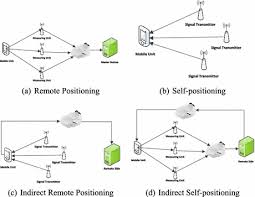
\includegraphics[width=0.6\textwidth]{img/topology}
  \caption{\label{fig:topology}Taxonomy of localization systems topology}
\end{figure}

\subsection{Coordinate System}
\begin{itemize}
  \item \textbf{Physical}: locations are represented as a point in a 2D/3D coordinate system;
  \item \textbf{Symbolic}: locations are expressed as logical positions’ information;
  \item \textbf{Absolute}: locations are expressed as unique coordinate values making reference to \textit{anchor} nodes that know their positions;
  \item \textbf{Relative}: locations are determined relatively to other nodes with no reference to absolute anchors.
\end{itemize}

\subsection{Communication paradigm}
\begin{itemize}
  \item \textbf{Non-cooperative}: the communication is restricted between unknown nodes and anchors (\textit{high density} of anchors or \textit{long-range anchor transmissions} are needed);
  \item \textbf{Cooperative}: allows communication between unknown nodes (more \textit{processing} is required);
  \item \textbf{Opportunistic}: exploits interactions between nodes that occasionally pass each other in their proximity (efficient \textit{node discovery} and \textit{data exchange}).
\end{itemize}

\subsection{Performance metrics}
\begin{itemize}
  \item \textbf{Accuracy}: mean (Euclidean) distance error between the estimated location and the true location;
  \item \textbf{Precision}: variation over many algorithm trials, CDF of distance error;
  \item \textbf{Complexity}: hardware and/or software;
  \item \textbf{Robustness}: behavior under unwanted conditions;
  \item \textbf{Scalability}: geographical and density;
  \item \textbf{Cost}
\end{itemize}

\subsection{Category}
The catogery of the localization technique pertains to how the location of a node is calculated depending on whether they are based on distance measurement or not. The two main categories are: \textit{range-based} and \textit{range-free}. 

Note that all the presented techniques are classified as \textit{anchor-based} schemes, assuming the existence of nodes with known positions.

\subsubsection{Range-based}
Range-based (or distance-based) techniques rely on the computation of distances between the target node and the anchor nodes to infer the position of a target node using \textit{lateration} techniques.

Location discovery consists of two phases:
\begin{enumerate}
  \item \textbf{Ranging phase} (or measuring distance): each node estimates its distance or angle from neighbors based on information contained in \textit{beacon} messages.
  The main three distance measuring methods are: 

  \begin{enumerate}[label=(\roman*)]
    \item \textit{Received Signal Strength (RSS)} estimates the distance from some set of neighbors using the attenuation of emitted signal strength. In free space, the RSS varies as the inverse square of the distance $d$ between the transmitter and the receiver:

    \begin{equation}
    P_r(d) = \frac{P_t G_t G_r \lambda^2}{(4\pi)^2 d^2}
    \end{equation}

    where $ P_r $ and $ P_t $ are respectively the reception and transmission power, $ G $ is the antenna gain, $ \lambda $ is constant and $ d $ is the distance between transmitter and receiver. Unfortunately, RSS is unreliable as it gets affected by the random multi-path effect.

    The parameters employed in these models are \textit{site-specific} and an empirical model is derived by obtaining a least square fit for each power level:

    \begin{equation}
    P_{RSSI} = \frac{X}{d^n}
    \end{equation}

    \item \textit{Time of Arrival} consists in calculating the one way propagation time of radio signals (RF) between two \textbf{synchronized} nodes. This time is proportional to the distance between transreceivers and is given by Eq.~\ref{eq:toa}:

    \begin{equation}
    d = c_r \times (t_1 - t_0)
    \label{eq:toa}
    \end{equation}

    This method of RF signals is usually inappropriate for WSNs because of short distances and inaccurate time synchronization of sensor nodes.

    \begin{figure}[b]
    \centering
    \begin{subfigure}{.5\textwidth}
      \centering
      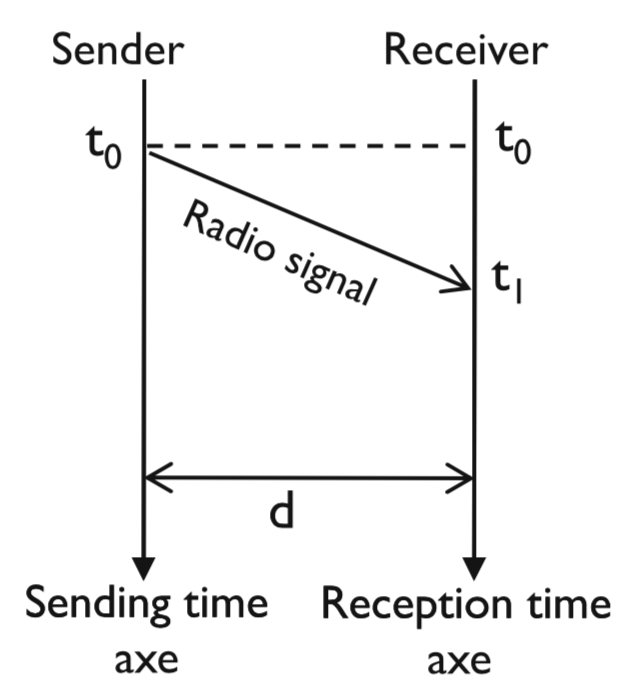
\includegraphics[width=.4\linewidth]{img/toa}
      \caption{Time of Arrival}
    \end{subfigure}%
    \begin{subfigure}{.5\textwidth}
      \centering
      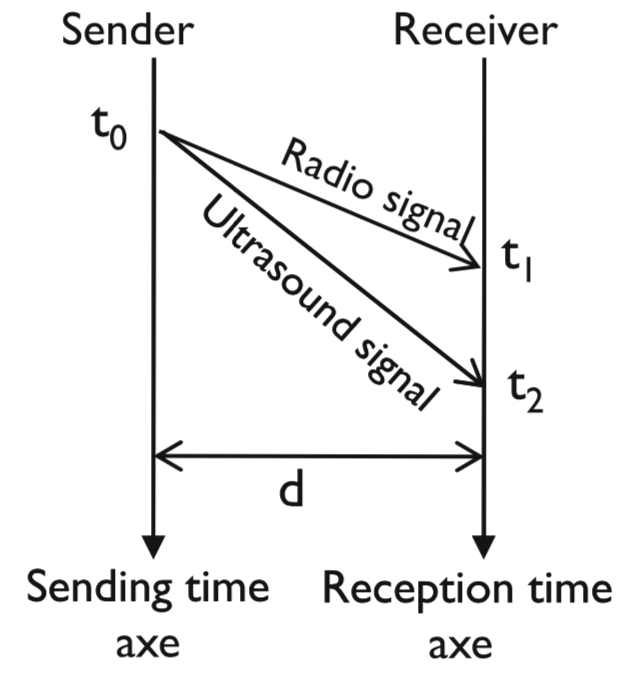
\includegraphics[width=.4\linewidth]{img/tdoa}
      \caption{Time Difference of Arrival}
    \end{subfigure}
    \caption{Time-based localization techiques}
    \end{figure}

    The TOA method can be used with Ultra-wideband (UWB) radio with which high accuracy can be achieved regardless the clock resolution thanks to the small propagation speed of ultrasound radios. This method is referred to as \textit{Time Difference of Arrival} (TDoA) and is based on the measurement of the time difference of the propagation of radio signals and ultrasound signals. When a node (anchor) simultaneously sends an RF signal and an ultrasound signal, the receiver (target) considers the arrival time of the (faster) radio signal as a time reference and uses the arrival time of the (slower) ultrasound radio to calculate the delay between the two signals. The distance is calculated according to Eq.~\ref{eq:tdoa}:

    \begin{equation}
    d = \frac{c_r \times c_u \times (t_2 - t_1)}{c_r - c_u}
    \label{eq:tdoa}
    \end{equation}

    where $c_r$ and $c_u$ are respectively the propagation speed of both radio and ultrasound signals, while $t_1$ and $t_2$ are their reception times at the receiver level.

    The TDOA method has the advantage to provide much better accuracy than RSS-based methods and it does not suffer from the need of explicit synchronization between nodes. However, it presents the drawback of requiring additional and more complex hardware with two different transceivers, which would have a negative impact on the cost.

    \item \textit{Angle of Arrival} relies on computing the angle by two lines connecting the unknown node with two anchor nodes. This technique relies on the use of directional antennas that can rotate on their axis or an array of antennas. For locating the unknown node at least three anchor nodes in 3D space and two anchor nodes in 2D space are needed.

    The advantage of AoA is that it does not require time sinchronization but on the other hand it requires vomplex and expensive hardware.
  \end{enumerate}

  \item \textbf{Estimation phase} (or combining distance): nodes use range information and anchors' locations to estimate their positions. In this phase some \textit{geometric geolocation techniques} are used:

  \begin{figure}[b]
    \centering
    \begin{subfigure}{.5\textwidth}
      \centering
      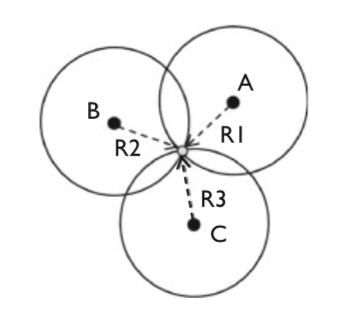
\includegraphics[width=.4\linewidth]{img/noise-free-lateration}
      \caption{with noise-free measurements}
    \end{subfigure}%
    \begin{subfigure}{.5\textwidth}
      \centering
      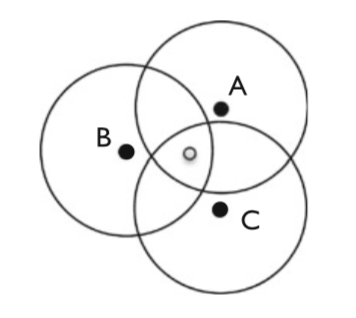
\includegraphics[width=.4\linewidth]{img/lateration}
      \caption{with noisy measurements}
    \end{subfigure}
    \caption{Trilateration technique}
  \end{figure}

  \begin{enumerate}[label=(\roman*)]
    \item \textit{Lateration/Trilateration} is the technique that uses distance information from anchor nodes to locate a target. In a 2D space, lateration involves the determination of the location of an unknown node as the intersection point of three circles centered in three non-collinear anchors (A, B and C), given that distances R1, R2 and R3 (i.e. circle radii) between the node and anchors are known. This technique is referred to as \textit{trilateration}. In a 3D space, there is a need of at least four anchor nodes to determine the location of a target node.
    \item \textit{Triangulation} is based on amgle measurements to estimate the location of an unknown node.
    \item \textit{Multi-lateration} takes in consideration more than the minimum number of required anchor nodes.
  \end{enumerate}
\end{enumerate}

\paragraph{Limitations}
Some of the analyzed range-based localization techniques are based on assumptions that do not always hold or are impractical such as circular radio range, symmetric radio connectivity, lack of obstructions, clear line-of-sight.

\subsubsection{Range-free}
Range-free methods do not rely on distance or angle estimation in localization. They rather use proximity or connectivity information to devise the location of the target.

Anchor-based range-free localization techniques can be classified as:
\begin{enumerate}[label=(\alph*)]
  \item \textit{Area-based approaches} estimate the position of the target as a particular point in the polygon formed by the anchor nodes. Two main method are proposed:
  \begin{enumerate}[label=(\roman*)]
    \item \textit{Centroid}
    \item \textit{Approximate Point-In-Triangle (APIT)}
  \end{enumerate}
  \item \textit{Multi-hop localization approaches} are used when a target is not in communication range with at least three anchor nodes because of the limitation of the transmission power. They rely on:
  \begin{enumerate}[label=(\roman*)]
    \item \textit{DV-Hop}
  \end{enumerate}
\end{enumerate}

\end{document}